
\noindent Working with nonabelian gauge theories, we've written down a Lagrangian density for Yang-mills theory, and after the gauge-fixing procedure of the Lagrangian density via path integrals and the tricks of Faddeev and Popov, we are ready to do some calculations. \\

\noindent The first topic to discuss is the \textit{beta function} or \textit{renormalization group equation}, which tells us how theories behave at low and high energies. The second topic to discuss is the departure from path integrals and gauge fixing to methods of lattice regulators, or cutoffs, for doing calculations in nonabelian gauge theory. \\

\subsection*{Renormalization of Nonabelian Gauge Theories}

\noindent We begin by reviewing renormalizability of quantum theories and the renormalization group equation, which tells us how coupling constants depend on the cutoff and how to adjust the coupling constants to match low and high energy predictions.  \\

\noindent Recall that a quantum theory $\hat{H}(z_1, \dots, z_n; \Lambda)$, where $\Lambda$ is the cutoff, data defined in a list of all the degrees of freedom of the theory, is renormalizable is it leads to finite predictions for all operationally well-defined observables. The expectation values of these observables must produce the same predictions for different choices of the chosen cutoff

\begin{equation}
\langle \hat{A}_j \rangle (z_1, \dots, z_n; K_c) \equiv f_j (z_1, \dots , z_n; K_c) = \alpha_j^{\text{obs.}}
\end{equation}

\noindent Where $K_c$ is a particular choice of cutoff: the length of list $\Lambda$, for example. This relationship of expectation values with different cutoffs yielding the same observed quantities is achieved in a renormalizable theory by allowing the coupling constants to depend on the cutoff $z_i  =z_i (K_c)$. \\

\noindent Apply the above equation to the Green's function, $n$-point correlation functions, where the dependency of the coupling constants and cutoff are implicit to the vacuum state $\ket{\Omega}$ and the dynamics of the field operators

\begin{align}
G^{(n)}(x_1, \dots, x_m; K_c) &\equiv \bra{\Omega} \mathcal{T} [\hat{\phi}(x_1) \dots \hat{\phi} (x_m) ] \ket{\Omega} \\
&\text{, where } \ket{\Omega} = \ket{\Omega(z_1, \dots , z_n; K_c)} \\
&\text{, and } \hat{\phi}(x) \equiv e^{-i \hat{H}(z_1, \dots, z_n; K_c)t} \hat{\phi}(0,\underline{x}) e^{i \hat{H}(z_1, \dots , z_n; K_c)t}.
\end{align}

\noindent So, we can equivalently say that a quantum theory $\hat{H}(z_1, \dots, z_n; \Lambda)$ is renormalizable if the correlation functions produce finite predictions for time-ordered quantities. \\

\noindent Now, to compute the relationship of $G^{(n)}$ to the coupling constants and the cutoff, consider changing the (usually) continuous parameter $K_c$ by an infinitesimal amount. Note that a common choice of cutoff could be $K_c = | p_{\text{max}} |$.

\begin{equation}
dG^{(n)} = \frac{\partial G^{(n)}}{\partial K_c} \delta K_c + \frac{\partial G^{(n)}}{\partial z_j} \delta z_j .
\end{equation}

\noindent So, the coupling constants $z_j (K_c)$ are chosen to fix $G^{(n)}$ with respect to transformations of the cutoff of the form $K_c \rightarrow K_c + \delta K_c$, but $G^{(n)}$ should not depend on $K_c$, and the above expression is equal to zero \\

\noindent To derive the \textit{renormalization group equation} or the \textit{beta function}, set the differential $dG^{(n)}$ to zero, divide by $\delta K_c$, and multiply by $K_c$

\begin{align}
\left[ K_c \frac{\partial}{\partial K_c} + K_c \frac{d z_j}{d K_c} \frac{\partial}{\partial z_j} \right] G^{(n)}&= 0 \\
\left[ K_c \frac{\partial}{\partial K_c} + \beta(z_j) \frac{\partial}{\partial z_j} \right] G^{(n)} &= 0 .
\end{align}

\noindent This is the infinitesimal form of the statement for a renormalizable theory that the Green's function shouldn't depend on the cutoff as it is changed, where 

\begin{equation}
\beta(z_j) = K_c \frac{d z_j}{d K_c} = \frac{d z_j}{d \, \text{ln} K_c}
\end{equation} 

\noindent Is the renormalization group or beta function, which allows us to compute the coupling constants in terms of the cutoff $z_j = z_j(K_c)$. The behavior of $\beta (z_j(K_c))$ is often used to describe the dependence of $z_j$ on $K_c$. \\

\subsection*{Aside: Massless Theories}

\noindent When we fix the Green's function to be equal to observable quantities, for any choice of cutoff, in a massive theory, we usually demand that the 2-point correlation function $\bra{\Omega} \hat{\phi} (p) \hat{\phi} (-p) \ket{\Omega}$ has a pole at the physical mass of the particle $m_{\text{phys}}$. \\

\noindent Complications arise in massless theories, as this leads to divergences, in the sense that we will end up with expressions like $\infty = \infty$. For massless theories, we instead insist that the 2-point correlation function has a pole at a negative, spacelike momenta $p^2 = -K_c^2 \equiv M^2$ with residue equal to one. This leads to finite predictions when we let $K_c \rightarrow \infty$.

\subsection*{Examples of Beta Functions}

\noindent (1) In $\phi^4$ theory, there is one coupling constant $\lambda$, the interaction strength, and the beta function is 

\begin{equation}
\beta(\lambda) = \frac{3 \lambda^2}{16 \pi^2} + \mathcal{O}(\lambda^3).
\end{equation}

\noindent (2) In quantum electrodynamics (QED), which is an abelian gauge theory, to first loop order, the beta function is 

\begin{equation}
\beta(e) = \frac{e^3}{12 \pi^2} + \mathcal{O}(e^4).
\end{equation}

\noindent Where $e$ is the electric charge of the particle. \\

\noindent (3) In Yang-Mills theory, a nonabelian gauge theory, there is more work to do in analyzing the divergences in the propagation of gauge bosons, as well as the propagation of fermions (quarks). The path integrals derived from applying the Yang-Mills theory Feynman rules produce divergences from the following terms in the Feynman expansion. See \textit{Peskin and Schroeder}, section 16.5 \textit{One-Loop Divergences of Non-Abelian Gauge Theory}, pages 521-544, for reference.

\begin{figure}[H]
	\centering
	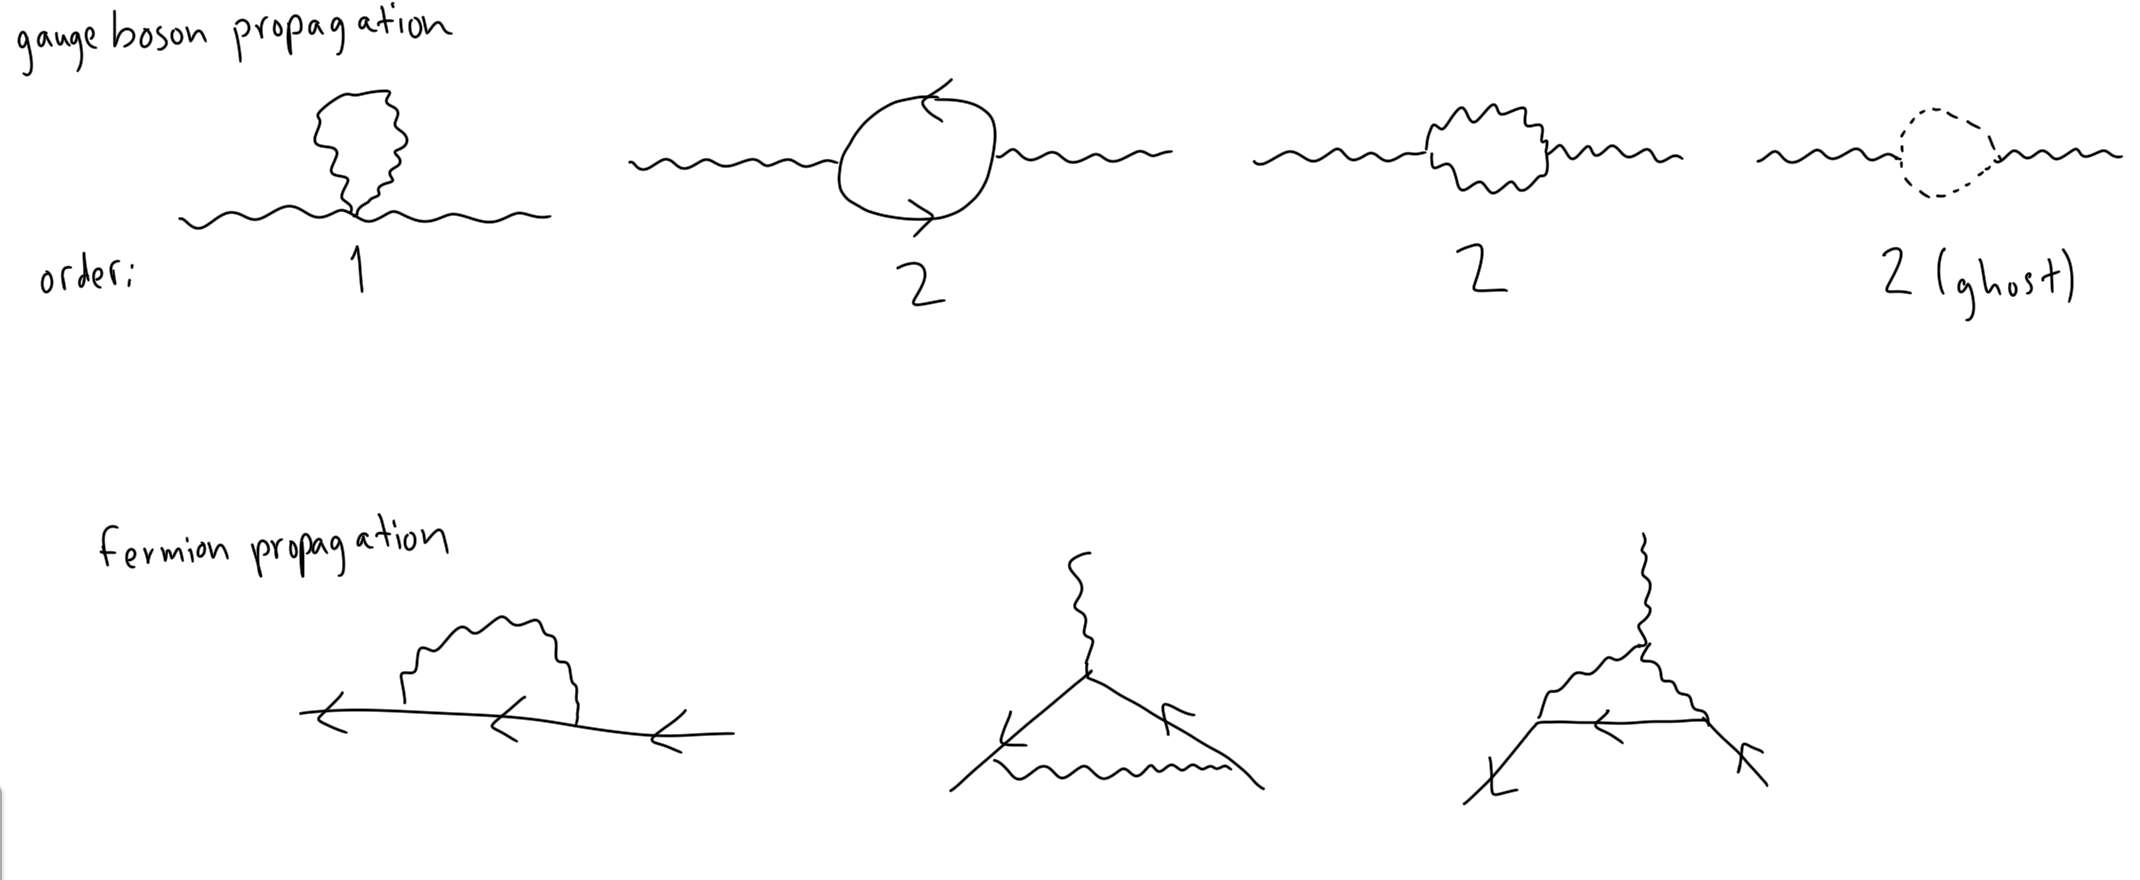
\includegraphics[width=5in]{images/beta_nagauge_div.png}
	\caption*{}
\end{figure}

\noindent To tame the infinities that arise from these diagrams, apply dimensional regularization to maintain Lorentz invariance and insist that each diagram leads to finite quantities. This then tells us what kinds of counter terms we need to add to the Lagrangian density for our theory, and, in turn, how the coupling constants change with respect to the cutoff. \\

\noindent This leads to the beta function for the $SU(N)$ local gauge group 

\begin{equation}
\beta(g) = - \frac{g^3}{16 \pi^2} \left( \frac{11 N}{3} - \frac{2 n_f}{3} \right)
\end{equation}

\noindent Where $n_f$ is the number of fermion families. Note that if $n_f$ is small, $\beta(g)$ becomes negative, and that $K_c \rightarrow \infty$ as $g$ gets smaller, meaning that our theory approaches being a free theory as $g \rightarrow 0$, and we can use perturbation theory for high-energy processes. This is called \textit{asymptotic freedom} of nonabelian gauge theories. \\

\subsection*{Low-Energy Physics of Nonabelian Gauge Theories}

\noindent Results here are thanks to Wilson's \textit{Confinement of Quarks} (1974). \\

\noindent To quantize an abelian or nonabelian gauge theory onto a discrete lattice, Wilson proposed the use of a lattice regulator. This is very challenging, since the gauge group acts on gauge fields like

\begin{equation}
A_\mu^j \frac{\sigma^j}{2} \rightarrow A_\mu^j \frac{\sigma^j}{2} + \frac{1}{g} (\partial_\mu \alpha^j) \frac{\sigma^j}{2} + i \left[\alpha^k \frac{\sigma^k}{2}, \alpha^l \frac{\sigma^l}{2}\right]
\end{equation}

\noindent And there any many complications in discretizing the derivative $\partial_\mu \alpha^j$ to the lattice. \\

\noindent Wilson recognized that the parallel transporter is the object that allowed us to do derivatives in the first place, and treated the parallel transporter 

\begin{equation}
U(j, j+\hat{e}^\mu) \in SU(2)
\end{equation}

as the fundamental degrees of freedom of the nonabelian gauge theory discretized to the lattice $\epsilon \mathbb{Z}^4$, instead of the gauge field.

\begin{figure}[H]
	\centering
	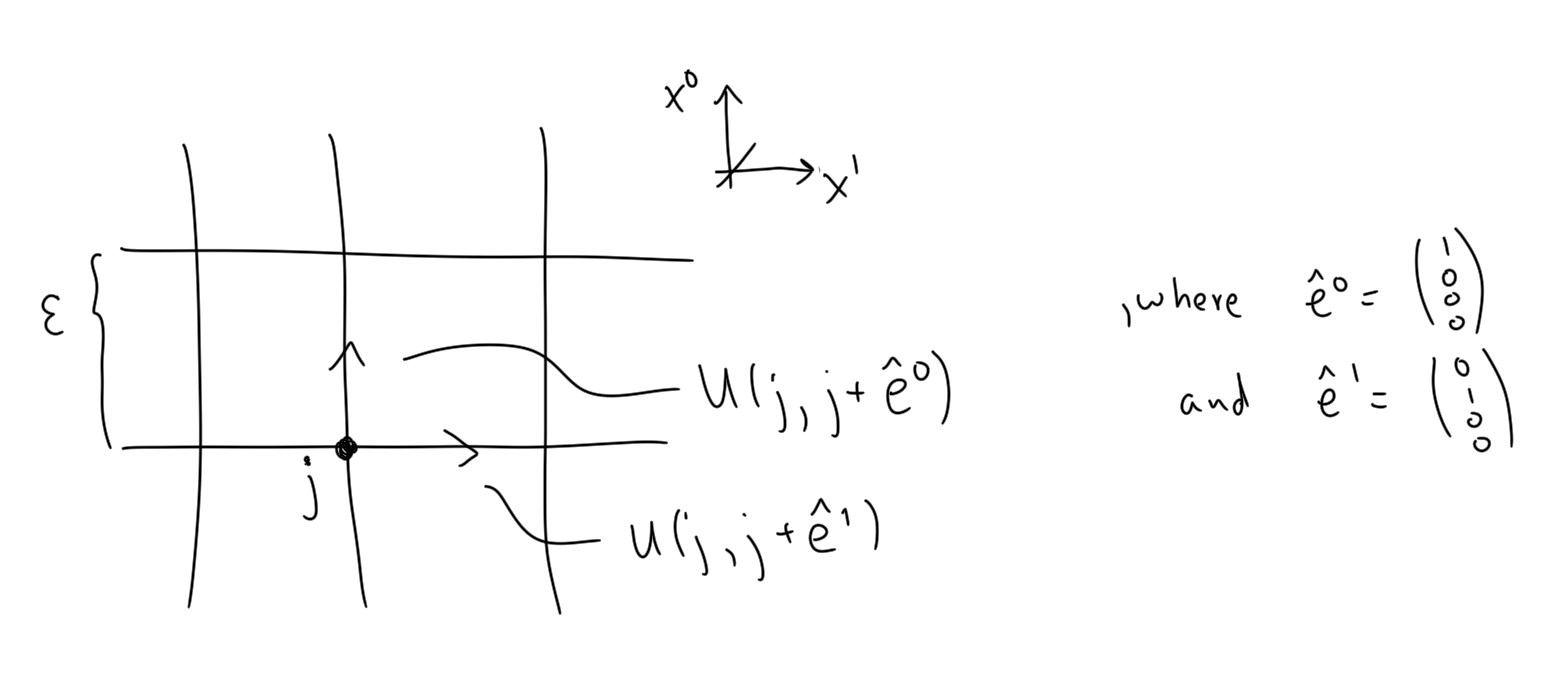
\includegraphics[width=4in]{images/wilson_parallel1.png}
	\caption*{}
\end{figure}

\noindent Bigger parallel transporters are built via multiplication. For example,

\begin{equation}
U(j, j+2\hat{e}^\mu) = U(j + \hat{e}^\mu, j+2\hat{e}^\mu)U(j, j+\hat{e}^\mu)
\end{equation}

\noindent These parallel transporters are $2 \times 2$ unitary matrices which populate the list of degrees of freedom, one for each link, or edge, in the classical lattice.\\

\noindent Side: Wilson ran calculations for the dynamics of a gauge field on a $4 \times 4 \times 4 \times 4$ lattice, which requires $4^4 \text{ lattice sites } \times 3 \text{ spatial coordinates per lattice site} = 768$ single-precision floating point numbers per unit time, requiring just 4 kilobytes of RAM. Note that a gigabyte ($\simeq 2^{30}$ bytes) of RAM is capable of storing $\sim 250,000,000$ single-precision floating point numbers, corresponding to almost $100 \times 100 \times 100 \times 100$ lattice. \\

\noindent To quantize the nonabelian gauge theory, Wilson proposed a way to build an action that summed over the plaquettes of the lattice, called \textit{Wilson loops}. In terms of the parallel transporters, the action has the form

\begin{equation}
S[U] = \sum_\Box \text{Wilson loops} = \sum_\Box \text{tr}(U_1 \cdot U_2 \cdot U_3 \cdot U_4)
\end{equation}

\noindent Where travelling around a plaquette may look like

\begin{figure}[H]
	\centering
	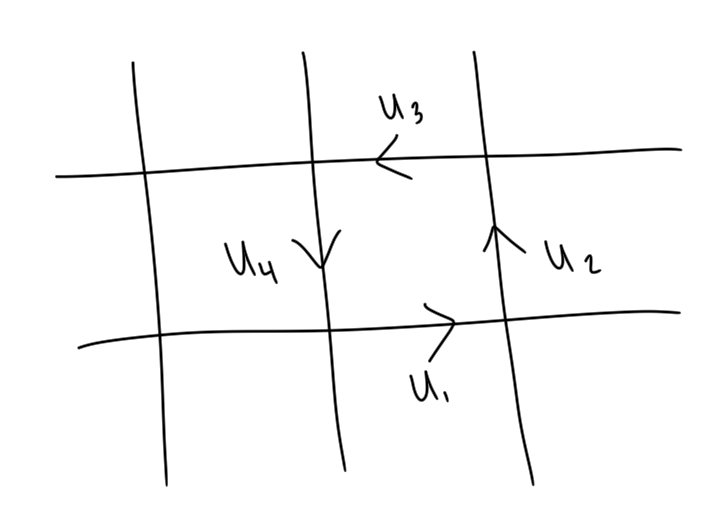
\includegraphics[width=2in]{images/wilson_parallel2.png}
	\caption*{}
\end{figure}

\noindent With this action, build the path integral $\int \mathcal{D}U \, e^{-iS[U]}$, and Wick rotate into the path integral $\int \mathcal{D}U \, e^{-S[U]}$ to work in imaginary time. Lastly, Monte Carlo sample the path integral. \\

\noindent This approach is actually the best way to get nonperturbative results in quantum field theory, but has its downsides: \\

\noindent Downside (1) is calculating processes in imaginary time is just like doing statistical mechanics with gauge theories at some defined temperature, and this is not good for time-ordered processes (e.g., scattering). Downside (2) is that this is not a quantum theory, as the Wilson loop is a classical configuration.

\subsection*{Hamiltonian Lattice Gauge Theory}

\noindent An alternative approach to quantization was introduced by Kogut and Susskind in 1975. They proposed a lattice quantum gauge theory, a quantum theory with a Hamiltonian and Hilbert space in which the degrees of freedom live on a lattice, which they argued yields Yang-Mills theory as the lattice spacing goes to zero. This is not proven, but if you can prove it, as well as that the low-energy limit has a mass cap, you can get a cool \$1M! \\

\noindent Recall that classically, each link, or edge, of the lattice is associated to a $2 \times2$ unitary matrix $U \in SU(2)$. In this lattice quantum gauge theory, each link or edge $e$ is associated to a wavefunction $\psi: \, SU(2) \rightarrow \mathbb{C}$, such that the wavefunction $\psi$ belongs the two-dimensional square-integrable functions on $SU(2)$ which is itself a Hilbert space per link $h_e$

\begin{equation}
\psi \in L^2 (SU(2)) \simeq h_e.
\end{equation}

\noindent Recall that $SU(2)$ is diffeomorphic to $S^3$, which conjures memories and solutions of wavefunctions on a sphere: spherical harmonics. \\

\noindent The total Hilbert space of this quantum theory is a tensor product over all the edges $e$ in the lattice $E$ of individual Hilbert spaces $h_e$

\begin{equation}
\mathcal{H} = \otimes_{e \in E} = \otimes_{e \in E} L^2 (SU(2)).
\end{equation}

\noindent To build the Hamiltonian, introduce some oeprations on the Hilbert space. First, write the states as kets in the position basis

\begin{equation}
\ket{\psi} = \int_{SU(2)} dU \, \psi (U) \ket{U}
\end{equation}

\noindent Where $\ket{U}$ is the position eigenvector defined by the three spatial coordinates. These states obey the inner product $\braket{U|V} = \delta(U-V)$. \\

\noindent Introduce the operators

\begin{equation}
L_U \ket{\psi} \equiv \int dV \, \psi (V) \ket{UV} \,\, \text{and} \,\, R_U \ket{\psi} \equiv \int dV \, \psi(V) \ket{VU^\dagger}.
\end{equation}

\noindent These operators are an analog of the shift operator $e^{ix \hat{p}}$. Note that $\ket{UV}$ is still a member of $SU(2)$. Differentiating these operators with respect to $U$ will yield momentum operators: dynamics.
